\documentclass[review]{elsarticle}

\usepackage{lineno,hyperref}
\modulolinenumbers[5]

\journal{Journal of Information and Software Technology}

\usepackage{subfig}
\usepackage{listings}
\usepackage[justification=raggedright, font=footnotesize, margin={10pt,0pt}]{caption}

\usepackage{minibox}
\usepackage{booktabs}
\usepackage{multirow}
\usepackage{ifthen}

\usepackage{comment}

\usepackage{amsbsy}
\usepackage{amssymb}
\usepackage{color}

\definecolor{backcolor}{gray}{0.9}

%\definecolor{lightgray}{rgb}{.9,.9,.9}

\definecolor{darkgray}{rgb}{.4,.4,.4}
\definecolor{purple}{rgb}{0.65, 0.12, 0.82}
\definecolor{darkgreen}{rgb}{0,0.4,0}

\lstdefinelanguage{JavaScript}{
	keywords={typeof, new, true, false, catch, function, return, null, catch, switch, var, let, if, in, while, do, else, case, break, constructor, class, extends, get, set, interface, const, public},
	keywordstyle=\color{blue}\bfseries,
	ndkeywords={export, throw, implements, import, this, require, super, prototype, void},
	ndkeywordstyle=\color{darkgray}\bfseries,
	identifierstyle=\color{black},
	sensitive=false,
	comment=[l]{//},
	morecomment=[s]{/*}{*/},
	commentstyle=\color{purple}\ttfamily,
	stringstyle=\color{red}\ttfamily,
	morestring=[b]',
	morestring=[b]"
}

\lstset{
	language=JavaScript,
	backgroundcolor=\color{backcolor},
	extendedchars=true,
	basicstyle=\footnotesize\ttfamily,
	showstringspaces=false,
	showspaces=false,
	numbers=left,
	numberstyle=\tiny,
	numbersep=4pt,
	xleftmargin= 10pt,
	tabsize=2,
	breaklines=true,
	showtabs=false,
	captionpos=b
}

\newcommand{\aspas}[1]{{``#1''}}
\newcommand{\mcode}[1]{$\tt #1$}

% comments \nb{label}{color}{text}
\newboolean{showcomments}
\setboolean{showcomments}{true}
\ifthenelse{\boolean{showcomments}}
	{\newcommand{\nb}[3]{
		{\colorbox{#2}{\bfseries\sffamily\scriptsize\textcolor{white}{#1}}}
		{\textcolor{#2}{\sf\small$\blacktriangleright$\textit{#3}$\blacktriangleleft$}}}
	 \newcommand{\version}{\emph{\scriptsize$-$Id$-$}}}
	{\newcommand{\nb}[3]{}
	 \newcommand{\version}{}}
\newcommand{\rev}[2]{\nb{Reviewer #1}{red}{#2}}
\newcommand{\ab}[1]{\nb{Alexandre}{blue}{#1}}
\newcommand{\lr}[1]{\nb{Lukas}{pink}{#1}}
\newcommand{\ai}[1]{\nb{Alejandro}{orange}{#1}}
\newcommand{\on}[1]{\nb{Oscar}{olive}{#1}}
\newcommand{\jk}[1]{\nb{Juraj}{orange}{#1}}
\newcommand{\rr}[1]{\nb{Romain}{red}{#1}}

% proof-reading
\usepackage{xcolor}
\usepackage[normalem]{ulem}
\newcommand{\ra}{$\rightarrow$}
\newcommand{\ugh}[1]{\textcolor{red}{\uwave{#1}}} % please rephrase
\newcommand{\ins}[1]{\textcolor{blue}{\uline{#1}}} % please insert
\newcommand{\del}[1]{\textcolor{red}{\sout{#1}}} % please delete
\newcommand{\chg}[2]{\textcolor{red}{\sout{#1}}{\ra}\textcolor{blue}{\uline{#2}}} % please change
\newcommand{\chk}[1]{\textcolor{ForestGreen}{#1}} % changed, please check


%%%%%%%%%%%%%%%%%%%%%%%
%% Elsevier bibliography styles
%%%%%%%%%%%%%%%%%%%%%%%
%% To change the style, put a % in front of the second line of the current style and
%% remove the % from the second line of the style you would like to use.
%%%%%%%%%%%%%%%%%%%%%%%

%% Numbered
%\bibliographystyle{model1-num-names}

%% Numbered without titles
%\bibliographystyle{model1a-num-names}

%% Harvard
%\bibliographystyle{model2-names.bst}\biboptions{authoryear}

%% Vancouver numbered
%\usepackage{numcompress}\bibliographystyle{model3-num-names}

%% Vancouver name/year
%\usepackage{numcompress}\bibliographystyle{model4-names}\biboptions{authoryear}

%% APA style
%\bibliographystyle{model5-names}\biboptions{authoryear}

%% AMA style
%\usepackage{numcompress}\bibliographystyle{model6-num-names}

%% `Elsevier LaTeX' style
\bibliographystyle{elsarticle-num}
%%%%%%%%%%%%%%%%%%%%%%%

\begin{document}

\begin{frontmatter}

\title{Using Facebook's Flow to Retrieve Class Dependencies in JavaScript: An Empirical Assessment}

%\tnotetext[mytitlenote]{Fully documented templates are available in the elsarticle package on \href{http://www.ctan.org/tex-archive/macros/latex/contrib/elsarticle}{CTAN}.}

%% Group authors per affiliation:
%\author{Elsevier\fnref{myfootnote}}
%\address{Radarweg 29, Amsterdam}
%\fntext[myfootnote]{Since 1880.}

%% or include affiliations in footnotes:
\author[mymainaddress]{Leonardo Humberto Silva\corref{mycorrespondingauthor}}
\cortext[mycorrespondingauthor]{Corresponding author}
\ead{leonardo.silva@ifnmg.edu.br}

\author[mtovaddress]{Marco Tulio Valente}
\ead{mtov@dcc.ufmg.br}

\author[bergeladdress]{Alexandre Bergel}
\ead{abergel@dcc.uchile.cl}

\address[mymainaddress]{Federal Institute of Northern Minas Gerais}
\address[mtovaddress]{Federal University of Minas Gerais}
\address[bergeladdress]{ISCLab, DCC, University of Chile}

\begin{abstract}
Accurately identifying dependencies between software components is an essential activity when maintaining and evolving software applications. It is also known that developers often use classes to tackle the complexity of legacy JavaScript code, \emph{i.e.}, code implemented in JavaScript versions that do not provide syntactical support to classes. In this scenario, identifying associations and other dependencies between classes is specially challenging due to the lack of types in the source code. This paper investigates the use of type inference to identify relationships between classes in legacy JavaScript code. We demonstrate how to use Flow, a static type-checker for JavaScript, to infer types that correspond to class references in systems transpiled from TypeScript to JavaScript. Our results show that precision reaches 100\% in the evaluated systems. Flow's recall ranges from 85\% to 96\% for associations, 64\% to 99\% for \aspas{uses} dependencies, and, if we consider both, from 80\% to 98\%. We manually analyzed and categorized all false negatives identified in our study. Finally, we successfully apply our approach in a set of vanilla JavaScript systems. The overall results suggest that using a type inferencer is a reliable approach to identify dependencies between software components in JavaScript.
%\ab{What is the take-away message? That using a type inferencer is a cheap and reliable approach to identify dependencies between software component? If yes, then say it}
%We find that the migration of legacy code to the new class syntax simplifies type inference and, by consequence, the identification of class-to-class dependencies. 
\end{abstract}

\begin{keyword}
JavaScript \sep Reverse engineering \sep Class dependencies \sep Flow
%\MSC[2010] 00-01\sep  99-00
\end{keyword}

\end{frontmatter}

\linenumbers

\section{Introduction}
\label{sec:introduction}

%\ab{The introduction can be a bit expanded to say how dependencies are usually inferred in other dynamically typed languages. For example, in Python, meta information provided by pip are used to retreive dependencies. In JavaScript, these metainformation are either provided by AMD, NPM...}

Highly-coupled systems, in which modules have unnecessary dependencies, are hard to maintain and evolve because these modules cannot be easily understood separately~\cite{Parnas1978, dsm}. The same rationale applies to class-to-class dependencies in object-oriented code. In some cases, an excessive number of class dependencies may be considered as an indicator of a poor software design. In JavaScript, the identification of such dependencies is specially challenging due to two main reasons: (i) the lack of types in the source code and (ii) the prototype-based mechanism of the language. However, even without native support, classes are often emulated in JavaScript using prototypes~\cite{silva-saner2015, gama:2012}. It is also important to mention that most of the JavaScript projects are currently implemented according to ECMAScript 5 (ES5), the last version of ECMAScript without class support, representing a large codebase of \textit{legacy} code that needs maintenance and evolution. The class syntax for JavaScript was introduced in version 6 of ECMAScript (ES6), released in the middle of 2015~\cite{ecmascript6}. In this paper, we employ the term \emph{legacy} to refer to applications implemented in JavaScript versions that do not use the syntactical support to classes introduced by ES6.

Module systems are the foundation of many design patterns and are critically necessary when building any non-trivial JavaScript-based application. The official JavaScript specification does not define a standard library that is useful for exporting module definitions. Looking at the ES5 module specifications, Asynchronous Module Definition (AMD)\footnote{\url{https://github.com/amdjs/amdjs-api/wiki}}  is popular among client-side code, while \mcode{CommonJS}\footnote{\url{http://www.commonjs.org/}} standard, which is implemented by \mcode{Node.js}, is the leading pattern in server-side environments. After the release of ES6, the specification of \aspas{ES6 modules} attempts to bridge the differences between AMD and \mcode{Node.js}, using a declarative syntax, for importing and exporting, and a programmatic loader API, to configure how modules are loaded and to conditionally load them. Other dynamically typed languages use similar standards to create dependencies between modules. For example, in Python, meta information provided by a package manager called \mcode{pip} are used to retrieve dependencies.\footnote{\url{https://docs.python.org/3/installing/index.html}}. In Ruby, each module defines a namespace and a sandbox in which methods and constants are encapsulated, similar to a class definition.\footnote{\url{https://ruby-doc.com/docs/ProgrammingRuby/html/tut_modules.html}}

Type information is essential to properly identify dependencies between class structures (or modules). These dependencies form the basis to provide, for example, class diagrams for JavaScript applications. Type inference is a known technique that identifies the type of variables using static code analysis. Some type inferencer tools have been proposed for JavaScript~\cite{odgaard-2014, Hack12a,Ande05a}. In this paper, we investigate the use of type inference to produce type information and unveil dependencies between classes. 

\begin{comment}

\begin{figure*}[ht]
	\centering
	
	\begin{minipage}{6.5in}
		\vspace*{0.10cm}
		%\centering
		\subfloat[\label{fig:DiagramNoDependencies}][Class diagram as currently identified by {\sc JSClassFinder}]{
			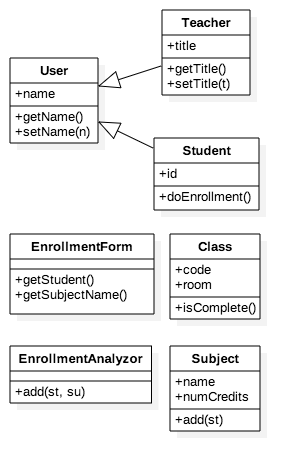
\includegraphics[width=0.31\textwidth]{fig/EnrollmentClassDiagramNoDependencies.png}}
		\subfloat[\label{fig:NewDiagram}][Class diagram with dependencies and types]{
			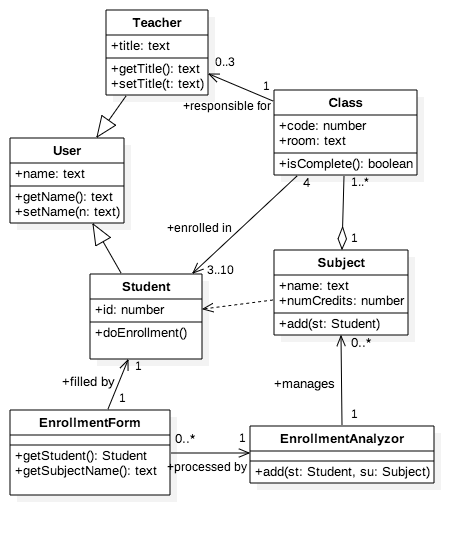
\includegraphics[width=0.46\textwidth]{fig/EnrollmentClassDiagram.png}}
		\vspace*{0.10cm}
	\end{minipage}
	\caption{Class diagrams for a simplified enrollment system in JavaScript\ab{I find this figure very weak. It simply shows, on a trivial example, a limitation of JSClassFinder. I think we can easily simply remove it.}}
	\label{fig:FutureClassDiagram}
\end{figure*}

\end{comment}

In a previous work~\cite{sanerera2017}, we presented a preliminary study to evaluate the use of Facebook's Flow\footnote{\url{https://flow.org/}}, a static type checker, to retrieve class-to-class dependencies in legacy JavaScript systems. We performed a study using code with and without annotating the class import statements in two modular applications. We achieved 100\% precision in the two analyzed systems, and recall ranging from 37\% to 51\% for dependencies in general and from 54\% to 85\% for associations, using type annotations for classes. In this paper, we extend their approach by preprocessing the source code in the \mcode{require} statements, eliminating variable references to class constructor functions implemented in other modules, instead of using type annotations for classes. This new approach increases recall, eliminates the need of annotating the source code, and allows the use of wildcards to import a set of classes in the same \mcode{require} statement. We analyze a set of systems transpiled from TypeScript to JavaScript and our results show that precision continues to be 100\%, and recall increases, reaching 99\% for \aspas{uses} dependencies and 96\% for associations, in the evaluated systems. We manually analyze and categorize all false negatives identified in our study. Our results suggest that: (i) inferencing types is key to extract inter-class dependencies in legacy JavaScript applications; (ii) Facebook's Flow represents a practical solution to extract dependencies from existing software and systems. Moreover, in a second study, we successfully identify class-to-class dependencies and associations on vanilla JavaScript projects by applying our approach. We find that the migration of legacy JavaScript code to the ES6 class syntax allows the use of name typing instead of structural typing, simplifying the type inference and, by consequence, the identification of class-to-class dependencies. 

%Besides the improvement in the values of recall, our approach does not require the migration of the constructor functions to use the new syntax for classes, introduced by ES6, in order to produce the type annotations for classes, as described in their preliminary work~\cite{sanerera2017}. 

The remainder of this paper is organized as follows. Section~\ref{sec:background} provides a background on class emulation in legacy JavaScript code, class dependencies, and type inference. Section~\ref{sec:approach} describes the methodology used to detect class-to-class dependencies in legacy JavaScript code. Section~\ref{sec:approach_es6} presents the benefits of name typing over structural typing when using Flow to infer types. Section~\ref{sec:study-design} describes the research questions that guide this work, along with the dataset and metrics used in our first study. We discuss answers to the proposed research questions in Section~\ref{sec:results} and explain the recall results in Section~\ref{sec:rq3-recall-results}. Section~\ref{sec:study-design-vanilla} demonstrates the application of our approach in a dataset of vanilla JavaScript systems. Threats to validity are exposed in Section~\ref{sec:threats} and related work is presented in Section~\ref{sec:related-work}. We conclude by summarizing our findings and discussing future work in Section~\ref{sec:conclusion}.
%We present a discussion about the lessons learned in Section~\ref{sec:discussion}. 


\section{Background}
\label{sec:background}

\subsection{Class Emulation in Legacy JavaScript Code}
\label{sec:class-emulation}

Functions are used to emulate classes in legacy JavaScript systems~\cite{leonardo-jsep2017, rostami2016}. Particularly, any function can be used as a template to create objects. When a function is used as a class constructor, the \mcode{this} variable is bound to the new object under construction. Variables linked to \mcode{this} are used to define properties that emulate attributes and methods. If a property is an inner function, it represents a {\em method}; otherwise, it is an {\em attribute}. The operator \mcode{new} is usually used to instantiate class objects. 

To illustrate the emulation of classes in legacy JavaScript code, we use a simple \mcode{Queue} class. Listing~\ref{lst_es5class} presents the code that defines this class, which includes a constructor function (lines 2-4), one attribute \mcode{\_elements} (line 3), and methods \mcode{isEmpty}, \mcode{push}, and \mcode{pop} (lines 5-7). 

\begin{figure}[htbp]
	\begin{lstlisting}[caption=Class emulation in legacy JavaScript code, label=lst_es5class]
// Class Queue
function Queue() { // Constructor function
	this._elements = new LinkedList();
}
Queue.prototype.isEmpty = function() {...}
Queue.prototype.push = function(e) {...}
Queue.prototype.pop = function() {...}
	\end{lstlisting}
\end{figure}

Indeed, the implementation in Listing~\ref{lst_es5class} represents one possibility of class emulation in JavaScript. Variations are possible, like implementing methods inside/outside class constructors and using anonymous/non-anonymous functions~\cite{silva-saner2015, gama:2012}.


\subsection{Class-To-Class Dependencies}
\label{subsec:dependencies}

Based on the UML specification~\cite{Fowler2003}, we consider two types of class-to-class dependencies in JavaScript: associations an dependencies of type \aspas{uses}. \textit{Associations} are particular cases of dependencies in which a class contains one or more attributes that are bound to instances of other classes. Figure~\ref{fig:example-associations} shows two examples of associations in JavaScript. In code (1), the constructor function for class \mcode{Z} is implemented in lines 6-8. The attribute \mcode{x}, which is part of class \mcode{Z}, receives an instance of class \mcode{X} (line 7), creating an association between the two classes. In code (2), the constructor function \mcode{Z} has a parameter \mcode{x} (line 6), which is assigned to the attribute \mcode{this.x} (line 7). In line 9, an instance of \mcode{Z} is created, with the parameter \mcode{x} bound to a newly created object of type \mcode{X}. If we consider the source code of the constructor functions, in code (1) we clearly notice the association between the two classes. However, in code (2), we need a client code (line 9), with the instantiation of classes \mcode{Z} and \mcode{X}, to establish the association.

\begin{figure}[ht]
	%\textit{Rule \#1: Class}\par\medskip
	%\vspace{-7pt}
	\centering
	\begin{minipage}{.35\textwidth}
		\begin{lstlisting}[backgroundcolor=\color{backcolor},numbers=left,frame=no,basicstyle=\ttfamily\footnotesize,xleftmargin=5pt,
		label={list:ex1_association},
		%caption={\em(before)},
		captionpos=b,
		title={(1)},
		emph={[2]},emphstyle={[2]\ttfamily\bfseries\color{black}},
		emph={[3]},emphstyle={[3]\ttfamily\bfseries\color{darkgreen}},
		emph={[4]},emphstyle={[4]\ttfamily\bfseries\color{orange}},
		emph={[5]getDate},emphstyle={[5]\ttfamily\bfseries\color{red}}]
// class X 
function X() {
	...
}
// class Z 
function Z() {
	this.x = new X();
}
...		
		\end{lstlisting}
	\end{minipage}
	\hspace{1pt}
	\begin{minipage}{.40\textwidth}
		\begin{lstlisting}[backgroundcolor=\color{backcolor},frame=no,numbers=left,basicstyle=\ttfamily\footnotesize,
		label={list:ex2_association},
		%caption={\em (after)},
		title={(2)},
		captionpos=b,
		emph={[2]},emphstyle={[2]\ttfamily\bfseries\color{black}},
		emph={[3]},emphstyle={[3]\ttfamily\bfseries\color{darkgreen}},
		emph={[4]},emphstyle={[4]\ttfamily\bfseries\color{orange}},
		emph={[5]},emphstyle={[5]\ttfamily\bfseries\color{red}}]
// class X 
function X() {
	...
}
// class Z
function Z(x) {
	this.x = x;
}
var z = new Z(new X());
		\end{lstlisting}
	\end{minipage}
	
	\caption{Examples of associations (from class \mcode{Z} to class \mcode{X})}
	\label{fig:example-associations}
\end{figure}

When a relationship between classes does not involve assignments of objects to class attributes, we have a \textit{uses} relationship, because one class just uses the other. Figure~\ref{fig:example-dependencies} shows two examples of dependencies in which a class \mcode{Z} \textit{uses} another class \mcode{X}. In code (1), we can see a method \mcode{foo} (lines 1-6) of a class \mcode{Z}. This method creates an instance of \mcode{X} and stores it in a local variable \mcode{\_x} for later use (line 4). In code (2), method \mcode{foo} receives an object as argument and \textit{uses} it to invoke its method \mcode{bar} (line 4). The identification of the class dependency is more challenging in code (2) because there is no direct reference to the \aspas{used} class in the source code of the method. 

\begin{figure}[ht]
	\centering
	\begin{minipage}{.35\textwidth}
		\begin{lstlisting}[backgroundcolor=\color{backcolor},numbers=left,frame=no,basicstyle=\ttfamily\footnotesize,xleftmargin=5pt,
		label={list:ex1_dependency},
		%caption={\em(before)},
		captionpos=b,
		title={(1)},
		emph={[2]},emphstyle={[2]\ttfamily\bfseries\color{black}},
		emph={[3]},emphstyle={[3]\ttfamily\bfseries\color{darkgreen}},
		emph={[4]},emphstyle={[4]\ttfamily\bfseries\color{orange}},
		emph={[5]getDate},emphstyle={[5]\ttfamily\bfseries\color{red}}]
Z.prototype.foo = 
	function() 
	{
		var _x = new X();
		...
	}  
		
		\end{lstlisting}
	\end{minipage}
	\hspace{1pt}
	\begin{minipage}{.40\textwidth}
		\begin{lstlisting}[backgroundcolor=\color{backcolor},numbers=left,frame=no,basicstyle=\ttfamily\footnotesize,xleftmargin=5pt,
		label={list:ex2_dependency},
		%caption={\em(before)},
		captionpos=b,
		title={(2)},
		emph={[2]},emphstyle={[2]\ttfamily\bfseries\color{black}},
		emph={[3]},emphstyle={[3]\ttfamily\bfseries\color{darkgreen}},
		emph={[4]},emphstyle={[4]\ttfamily\bfseries\color{orange}},
		emph={[5]getDate},emphstyle={[5]\ttfamily\bfseries\color{red}}]
Z.prototype.foo = 
	function(x) 
	{
		var _bar = x.bar();
		...
	}
		
		\end{lstlisting}
	\end{minipage}
	
	\centering\caption{Examples of dependencies of type \aspas{uses}}
	\label{fig:example-dependencies}
\end{figure}


In the remaining of this paper, the term dependency is used generically to reference both associations and dependencies of the type \textit{uses}.


\subsection{Type Inference}
\label{subsec:type-inference}

A type is a collection of program entities that share common properties. In general, we refer to the process of reasoning about unknown types as \textit{type inference}~\cite{Palsberg:1991}. A type inference mechanism analyzes the static structure of a program to infer the types of some or all of its expressions. Commonly, a type checker verifies if all the types are properly defined and used according to the semantics of the programming language. Statically typed languages, such as Java and C++, perform type checking at compile-time, demanding the developers to explicitly declare the types in the source code. Dynamically typed programming languages, such as JavaScript and Smalltalk, only check types at runtime. 

Flow\footnote{\url{http://flowtype.org/}} is a static type checker for JavaScript designed by Facebook. It employs a control-flow analysis that compilers typically perform to extract semantic information from code, and then uses this information for type inference. Listing~\ref{lst_flow} is one example of code in which Flow can detect incompatible types involving an expression (line 3) and the type passed as argument of the function call (line 5). Listing~\ref{lst_flow-feedback} shows the result of applying Flow to the code in Listing~\ref{lst_flow}. As we can see, Flow indicates a type error in the code of line 3 (a string is used as an operand in a multiplication).

%\vspace{5.5 mm}

\begin{lstlisting}[caption=Example of incompatible types detected by Flow, label=lst_flow]
// Function foo expects a number as argument
function foo(x) {  
	return x * 10;
}
foo('Hello, Flow!');
\end{lstlisting} 

\begin{lstlisting}[caption=Warning messages from Flow for the code in Listing~\ref{lst_flow}, label=lst_flow-feedback]
foo.js:5
5: foo('Hello, Flow!');
^^^^^^^^^^^^^^^^^^^ function call
3: 	return x * 10;
^ string. This type is incompatible with
3: 	return x * 10;
^^^^^^ number
\end{lstlisting} 

\vspace{1.0 mm}

Developers can also use type annotations to document their systems and to help Flow during type checking, although this is not mandatory.


\section{Using Flow to Infer Dependencies}
\label{sec:approach}

In this section, we describe the usage of a static type checker (Facebook's Flow) to identify dependencies between classes in legacy JavaScript code. The idea of using Flow as a type inferencer was originally introduced in our preliminary study to identify class-to-class dependencies~\cite{sanerera2017}. In this paper, we extend the initial approach by preprocessing the source code in the \mcode{require} statements, \emph{i.e.}, statements used to import source code definitions from other files, eliminating variable references to class constructor functions implemented in other modules. Figure~\ref{fig:proposed-approach} presents an overview of this new methodology. Given a JavaScript application, we infer dependencies as described next.

% I used the site draw-io to create the flow chart of figure \label{fig:proposed-approach}
\begin{figure*}[ht]
	\centering
	\captionsetup{justification=centering}
	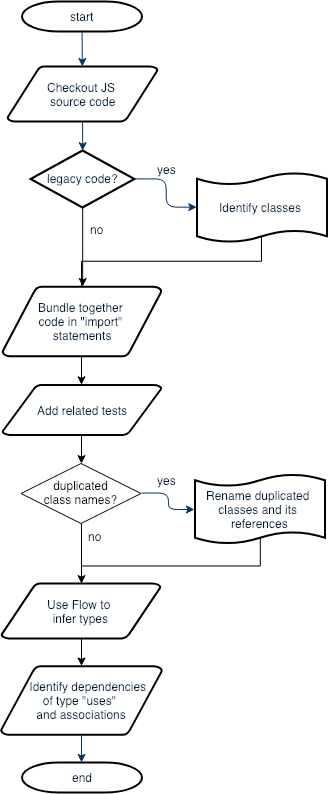
\includegraphics[width=12.3cm]{fig/flowchart_draw-io.png}
	\caption{Overview of the evaluated approach}
	\label{fig:proposed-approach}
\end{figure*}

\vspace{2.5 mm}

\noindent \textit{Class identification in case of legacy code.} In this step, we identify the classes emulated in a legacy JavaScript codebase using JSClassFinder~\cite{silva-cbsoft2015, leonardo-jsep2017}, which is a tool designed to detect classes in legacy JavaScript code. JSClassFinder works on the application's abstract syntax tree that is generated after pre-processing the source code. The tool then applies a set of heuristics to identify classes, methods, and attributes.%~\cite{leonardo-jsep2017}. 

\vspace{2.5 mm}

\noindent \textit{Bundle together code in \mcode{require} statements.} We bundle together files that depend on each other and use it as input for the type inferencer tool. 

\vspace{2.5 mm}

\noindent \textit{Add related tests.} We infer types passing the application's source code and tests as input. In this case, the tests are important to determine some of the types involved in class instantiations and method calls, like in the association showed in code (2) of Figure~\ref{fig:example-associations}.

\vspace{2.5 mm}

\noindent \textit{Rename duplicated class names and their references.} After bundling together the necessary files, \emph{i.e.}, related classes an tests, we look for duplicated class names in order to eliminate any ambiguity during the type inference process.  

\vspace{2.5 mm}

\noindent \textit{Use Flow to infer types.} Flow is a very active open source project, with more than 582 contributors, 8,054 commits, and almost 19K stars (data collected in January 2019).\footnote{\url{https://github.com/facebook/flow}} We execute Flow passing the application's source code and tests as input. The output produced by Flow is a text file that contains the coordinates (line, column) for every element of the source code (variable, function, object, etc), and their respective types. Figure \ref{fig:example-flow-point} shows the emulation of a simple class \mcode{Point} (code on the left) and the correspondent Flow's output (text on the right). We can see that there is a function in line 1 of the output file, denoted by the arrow (\aspas{=$>$}), whose name is located in line 4 of the file \mcode{Point.js}, between columns 10 and 14. This function has two arguments (\mcode{x} and \mcode{y}) of type \mcode{number} and returns \mcode{void}. Every time the keyword \mcode{this} is used, Flow infers the structure of the object that it represents as its type. For example, the structure of the object \mcode{this} that appears in lines 5 and 6 of the legacy code is \mcode{\{x:number, y:number\}} (see lines 4 and 7 of Flow's output file). In this case, the inferred object represents the attributes of \mcode{Point}. In other words, when a reference to an emulated class is found, Flow infers the structure of the object that represents the class as its type. 

\begin{figure*}[ht]
	\centering
	\begin{minipage}{.32\textwidth}
		\begin{lstlisting}[backgroundcolor=\color{backcolor},numbers=left,frame=no,basicstyle=\ttfamily\scriptsize,xleftmargin=5pt,
		label={list:ex1_dependency},
		%caption={\em(before)},
		captionpos=t,
		title={\mcode{Point.js}},
		emph={[2]},emphstyle={[2]\ttfamily\bfseries\color{black}},
		emph={[3]},emphstyle={[3]\ttfamily\bfseries\color{darkgreen}},
		emph={[4]},emphstyle={[4]\ttfamily\bfseries\color{orange}},
		emph={[5]getDate},emphstyle={[5]\ttfamily\bfseries\color{red}}]
/*
	Constructor function
*/
function Point (x, y) {
	this.x = x;
	this.y = y;
}	
		
/*
	Method getX()
*/ 
Point.prototype.getX = 
	function() {
		return this.x;
	}
		
// Creating an instance 
var p = new Point(2,3);
		\end{lstlisting}
	\end{minipage}
	\begin{minipage}{.02\textwidth}
		\raggedleft{$\Rightarrow$}
	\end{minipage}
	\hspace{3pt}
	\begin{minipage}{.60\textwidth}
		\begin{lstlisting}[backgroundcolor=\color{backcolor},numbers=left,frame=no,basicstyle=\ttfamily\scriptsize,xleftmargin=5pt,
		label={list:ex2_dependency},
		%caption={\em(before)},
		captionpos=t,
		title={Flow's output (text file with types)},
		emph={[2]},emphstyle={[2]\ttfamily\bfseries\color{black}},
		emph={[3]},emphstyle={[3]\ttfamily\bfseries\color{darkgreen}},
		emph={[4]},emphstyle={[4]\ttfamily\bfseries\color{orange}},
		emph={[5]getDate},emphstyle={[5]\ttfamily\bfseries\color{red}}]
Point.js:4:10-14: (x:number, y:number)=>void
Point.js:4:17: number
Point.js:4:20: number
Point.js:5:2-5: {x:number, y:number}
Point.js:5:2-11: number
Point.js:5:11: number
Point.js:6:2-5: {x:number, y:number}
Point.js:6:2-11: number
Point.js:6:11: number
Point.js:12:1-5: (x:number, y:number)=>void
Point.js:12:1-15: {getX: () => }
Point.js:12:1,15:2: () => 
Point.js:13:2,15:2: () => 
Point.js:14:13-16: 
Point.js:14:13-18: 
Point.js:18:5: {x:number, y:number}
Point.js:18:9-22: {x:number, y:number}
Point.js:18:13-17: (x:number, y:number)=>void
Point.js:18:19: number
Point.js:18:21: number
		
		\end{lstlisting}
	\end{minipage}
	
	\centering\caption{Example of Flow's output file}
	\label{fig:example-flow-point}
\end{figure*}

\vspace{3.0 mm}

In JavaScript, the value of \mcode{this} depends on how a function is called, and it may be different each time the function is called.\footnote{https://developer.mozilla.org/en/docs/Web/JavaScript/Reference/Operators/this}
For this reason, we do not have the return type of function \mcode{getX} in line 11 of the output file. In this case, since \mcode{getX} is not invoked in the code, Flow does not infer neither its return type nor the type of \mcode{this.x}, used in \mcode{getX} (lines 11-15 of the output file). To overcome this problem, it is important to pass the tests together with the source code as input for Flow, using as many function invocations as possible. If we add a call to \mcode{getX} at the end of the source code on the left, for example \mcode{p.getX()}, then Flow gives the following output: \mcode{{getX: ()=> number}}, identifying the return type as \mcode{number}.

\vspace{2.0 mm}

\noindent \textit{Identify dependencies of type \aspas{uses} and associations.} The classes identified in the source code and the types inferred by Flow are combined to infer dependencies, identifying which types represent class references. For JavaScript legacy code, we use structural equivalence to identify associations and \textit{uses} dependencies, since Flow infers the structures of objects, including class instances, as their types. In structural equivalence, two values have equivalent types if the types have isomorphic structures~\cite{connor90}. On the other hand, if the source code uses the class syntax (ES6+), class names are used as types and we can use name equivalence to locate class references.


\section{Using Flow to Infer ES6 Class Dependencies}
\label{sec:approach_es6}
%The use of structural typing becomes an obstacle when we move to larger systems. To favor the scalability of our approach, it would be important to be able to use name equivalence when looking for specific types. To achieve that, we propose the migration of class structures to ES6 syntax instead on working directly on the legacy code. 

When we apply Flow to a code written in ES6, the class names are recognized as types, and we can use name equivalence to compare these types. As an example, consider the code presented in Figure \ref{fig:example-flow-point}. If we rewrite the class \mcode{Point} according to ES6 syntax, and apply Flow, we will have an output file similar to the one in Figure \ref{fig:example-flow-point-es6}. In this case, we can see the class name as a type, instead of the structure of the object. In lines 1 and 14 of the output file, we can see the type \mcode{[class: Point]}, indicating that it represents the class declaration or one direct reference to the class name. In lines 4, 7, 10, 12 and 13, we can see the type \mcode{Point}, indicating the occurrence of an instance of the class \mcode{Point} in the source code. 
 
\begin{figure*}[ht]
	\centering
	\begin{minipage}{.32\textwidth}
		\begin{lstlisting}[backgroundcolor=\color{backcolor},numbers=left,frame=no,basicstyle=\ttfamily\scriptsize,xleftmargin=5pt,
		label={list:ex1_dependency},
		%caption={\em(before)},
		captionpos=t,
		title={\mcode{Point.js}},
		emph={[2]},emphstyle={[2]\ttfamily\bfseries\color{black}},
		emph={[3]},emphstyle={[3]\ttfamily\bfseries\color{darkgreen}},
		emph={[4]},emphstyle={[4]\ttfamily\bfseries\color{orange}},
		emph={[5]getDate},emphstyle={[5]\ttfamily\bfseries\color{red}}]
/*
	Class declaration
*/
class Point {
	constructor(x, y) {
		this.x = x;
		this.y = y;
	}	
		
	/*
		Method getX()
	*/ 
	getX() {
		return this.x;
	}
}	
	
// Creating an instance 
var p = new Point(2,3);
		\end{lstlisting}
	\end{minipage}
	\begin{minipage}{.02\textwidth}
		\raggedleft{$\Rightarrow$}
	\end{minipage}
	\hspace{3pt}
	\begin{minipage}{.60\textwidth}
		\begin{lstlisting}[backgroundcolor=\color{backcolor},numbers=left,frame=no,basicstyle=\ttfamily\scriptsize,xleftmargin=5pt,
		label={list:ex2_dependency},
		%caption={\em(before)},
		captionpos=t,
		title={Flow's output (text file with types)},
		emph={[2]},emphstyle={[2]\ttfamily\bfseries\color{black}},
		emph={[3]},emphstyle={[3]\ttfamily\bfseries\color{darkgreen}},
		emph={[4]},emphstyle={[4]\ttfamily\bfseries\color{orange}},
		emph={[5]getDate},emphstyle={[5]\ttfamily\bfseries\color{red}}]
Point.js:4:1,16:1: [class: Point]
Point.js:5:14: number
Point.js:5:17: number
Point.js:6:3-6: Point
Point.js:6:3-12: number
Point.js:6:12: number
Point.js:7:3-6: Point
Point.js:7:3-12: number
Point.js:7:12: number
Point.js:14:13-16: Point
Point.js:14:13-18: 
Point.js:19:5: Point
Point.js:19:9-22: Point
Point.js:19:13-17: [class: Point]
Point.js:19:19: number
Point.js:19:21: number
		
		\end{lstlisting}
	\end{minipage}
	
	\centering\caption{Example of Flow's output file for ES6 code}
	\label{fig:example-flow-point-es6}
\end{figure*}

The migration to ES6 classes and, by consequence, the use of name typing, simplifies the identification of class-to-class dependencies and allows the use of the proposed approach in larger systems. However, the migration of ES5 to ES6 classes can be challenging and risky, as we presented in a previous study~\cite{icsr2017}. In the next section we present the design of a study that uses structural equivalence to identify class dependencies in JavaScript legacy code.

%In Section~\ref{sec:study-design} we present the design of a study that uses structural equivalence to identify class dependencies in JavaScript legacy code. In Section~\ref{sec:study-design-vanilla} we identify dependencies in JavaScript systems using ES6 classes and name equivalence.

%:%%%%%%%%%%%%%%%%%%%%%%%%%
\section{Evaluation Design}
\label{sec:study-design}

In this section, we detail the design of a study proposed to evaluate the usage of Flow to detect dependencies between classes in legacy JavaScript systems. First, we present the metrics adopted to measure class-to-class dependencies in Section \ref{subsec:metrics}. The dataset and the oracle we use are described in Section \ref{subsec:dataset-oracle}. Then, we present the research questions that guide this study in Section \ref{subsec:rqs}.

\subsection{Class-Diagram Scope Metrics}
\label{subsec:metrics}

Although many metrics have been proposed for measuring object-oriented software systems, there are only a
few metrics for class diagrams~\cite{yi2004,genero2005}. These measures can be useful to predict class diagram external quality characteristics, such as maintainability~\cite{genero2002a, genero2005}. Genero et al.~\cite{genero2001, genero-phd-2002} defined a set of metrics to measure the structural complexity of a class diagram. Among these class-diagram scope metrics, we present the ones directly related to class-to-class dependencies:

\begin{itemize}
	\item \textit{NAssoc} - The total number of associations.
	\item \textit{NAgg} - The total number of aggregation relationships within a class
diagram (each whole-part pair in an aggregation relationship).
	\item \textit{NDep} - The total number of dependency relationships.
	\item \textit{NGen} - The total number of generalization relationships
within a class diagram (each parent-child pair in a
generalisation relationship).
	\item \textit{NgenH} - The total number of generalizations hierarchies in a class
diagram.
\end{itemize} 
%	\item \textit{NAssoc} - Association relationships. Representing the number of associations between classes.
%\item \textit{NDep} - Dependency relationships. Representing the number of dependencies of type \aspas{uses} between classes.

In this paper, we are collecting information about associations and dependencies of type \aspas{uses}. We are using the metric \textit{NAssoc}, for associations, and, since we do not measure aggregations separately, the \aspas{uses} dependencies include both: \textit{NAgg} and \textit{NDep}. Once generalizations are not included in our measures for \aspas{uses} dependencies, \textit{NGen} and \textit{NgenH} are not being used.  

For the sake of simplicity, we are introducing a metric called \textit{NUsesDep}, which represents the sum of Genero's metrics \textit{NAgg} and \textit{NDep}.

\vspace{2.5 mm}

\[
\textit{NUsesDep} = \textit{NAgg} + \textit{NDep}
\]

\vspace{3.0 mm}

%In, P., Kim, S., Barry, M. (2003): UML-based object-oriented metrics for
%architecture complexity analysis. Department of computer science, Texas
%A&M University, 2003. http://faculty.cs.tamu.edu/hohin

\subsection{Dataset and Oracle}
\label{subsec:dataset-oracle}

%\noindent \textit{Dataset and the oracle.} 
For our study, we need systems that emulate classes in legacy JavaScript in order to find the dependencies between these classes. We also need an oracle of class dependencies to measure the accuracy of the types inferred by Flow. For these reasons, we use TypeScript open-source projects to build this oracle and minimize possible bias. TypeScript is an extension of JavaScript that offers classes, interfaces, and a gradual type system~\cite{nance2014}. Therefore, by parsing and extracting explicit types in TypeScript programs, class-to-class dependencies can be found and added to an oracle. Before performing our analyses, TypeScript code is \textit{transpiled}\footnote{A transpiler is a source-to-source compiler. Transpilers are used, for example, to convert from TypeScript to JavaScript, in order to guarantee compatibility with existing browsers and runtime tools.} to vanilla JavaScript. The automatically generated code contains all constructor functions and methods, along with their dependencies, implemented according to JavaScript ES5 syntax. The strategy of using TypeScript projects to build an oracle is also adopted by Rostami \emph{et al.} \cite{rostami2016} in their work to detect constructor functions in JavaScript and by Silva \emph{et al.}~\cite{sanerera2017} in our preliminary study that evaluates the use of Flow as a type checker.
%, and by Silva \emph{et al.} \cite{sanerera2017} in their study to identify dependencies between classes in legacy JavaScript code. 

Table~\ref{tab:dataset} presents the main characteristics of the three TypeScript projects in our dataset, including version number, size (LOC), number of classes, number of dependencies of type \aspas{uses} (\textit{NUsesDep}), number of class associations (\textit{NAssoc}), and the total of dependencies. The information about the dependencies can be obtained directly by analyzing the TypeScript code, which has explicit types. {\sc inversifyjs}\footnote{\url{https://github.com/inversify/InversifyJS}} is a lightweight inversion of control container for TypeScript and JavaScript applications. {\sc satellizer}\footnote{\url{https://github.com/sahat/satellizer}} is an end-to-end token-based authentication module for \mcode{AngularJS} with built-in support to different service providers. {\sc xstream}\footnote{\url{http://staltz.com/xstream/}} is a fast functional reactive stream library for JavaScript. {\sc inversifyjs} and {\sc satellizer} are also used in our preliminary study~\cite{sanerera2017}.


\begin{table}[!ht]
	\scriptsize	
	\centering
	\caption{\textsc{Characteristics of the analyzed TypeScript systems}}
	\tabcolsep=0.11cm
	\begin{tabular}{lrrr|ccc}
		\toprule
		\multicolumn{4}{c|}{\textbf{Systems}} & \multicolumn{3}{c}{\textbf{Dependencies}}  \\
		Name & Version & LOC & Classes & \textit{NUsesDep} & \textit{NAssoc} & TOTAL  \\
		\midrule
		{\sc inversifyjs} & 2.0.1   & 1,527 &         20 & 134 & 26 & 160  \\
		{\sc satellizer}   & 0.15.5 &   990 &          11 & 19 & 20 & 39  \\
		{\sc xstream}    &  11.0.0 & 1,737 &         25 & 80 &  44 & 124  \\
		\bottomrule
	\end{tabular}
	\label{tab:dataset}
\end{table}

%\end{comment}


Listing~\ref{lst_typescript_inversifyjs} shows a simple class-based example in TypeScript. We can see explicit type annotations in attributes (line 2), which are used to infer associations, and in parameters (lines 4) and return types (line 8), which are used to infer \textit{uses} relations when building the oracle of class dependencies. % used in this chapter. 

\begin{lstlisting}[caption=Example of class in TypeScript, label=lst_typescript_inversifyjs, emph={[2]string,boolean},emphstyle={[2]\ttfamily\bfseries\color{darkgreen}}]
class Greeter {
	private greeting: string;

	constructor(message: string) {
		this.greeting = message;
	}
	
	public greet(): string {
		return "Hello, " + this.greeting;
	}
}  
\end{lstlisting} 

\vspace{2.0 mm}

Listing \ref{lst_typescript_kernel} shows a second example that contains class associations in {\sc inversifyjs}. The import statements (lines 1-3) link the variables (\mcode{Planner}, \mcode{Resolver}, and \mcode{Lookup}) to the respective classes, implemented in other files. Lines 5-19 contain the implementation of class \mcode{Kernel}, whose attributes are defined in lines 6-9 and initialized in the constructor function (lines 12-17). The attributes \mcode{\_planner}, \mcode{\_resolver}, and \mcode{\_bindingDictionary} receive new instances of the classes \mcode{Planner}, \mcode{Resolver}, and \mcode{Lookup}, respectively (lines 14-16). Therefore, we count three class associations in this example.

\vspace{6.0 mm}

\begin{lstlisting}[caption=Example of class associations in TypeScript, label=lst_typescript_kernel, basicstyle=\ttfamily\footnotesize, emph={[2]},emphstyle={[2]\ttfamily\bfseries\color{darkgreen}}]
import Planner from "../planning/planner";
import Resolver from "../resolution/resolver";
import Lookup from "./lookup";

class Kernel {
	public guid: string;
	private _planner: Planner;
	private _resolver: Resolver;
	private _bindingDictionary: Lookup<Binding<any>>;

	// Initialize private properties
	public constructor() {
		this.guid = guid();
		this._planner = new Planner();
		this._resolver = new Resolver();
		this._bindingDictionary = new Lookup<Binding<any>>();
	}
	...
}
\end{lstlisting} 

TypeScript language also supports the definition of interfaces to enforce certain properties on an object (class).
Listing~\ref{lst_typescript_interface} shows an example of an interface, called \mcode{Producer}, in system {\sc xstream}. This interface specifies the signatures for methods \mcode{start} and \mcode{stop}, that must be implemented by all \aspas{producers} in the system. 

\begin{lstlisting}[caption=Example of interface in TypeScript, label=lst_typescript_interface, basicstyle=\ttfamily\footnotesize, emph={[2]string,boolean},emphstyle={[2]\ttfamily\bfseries\color{darkgreen}}]
interface Producer<T> {
	start: (listener: Listener<T>) => void;
	stop: () => void;
}
\end{lstlisting} 

As in other languages that support interfaces, a property whose type is an interface can receive, at runtime, instances of classes that implement the interface. This does not represent a problem to the use of Flow to infer types of such properties for two reasons: (i) interfaces are part of the TypeScript syntax but they are not transpiled to JavaScript, having zero runtime impact; (ii) Flow is able to infer multiples types for the same property when this property receives objects of different types during execution. For example, if we have two classes \mcode{C1} and \mcode{C2} that implement the same interface \mcode{Producer}, Flow can infer the type \aspas{structure of \mcode{C1} $|$ structure of \mcode{C2}} for a property whose type in TypeScript is \mcode{Producer}. It depends on the values this property receives at runtime.

Another TypeScript feature that has no impact in the transpiled code is the use of \textit{type casting}. Listing~\ref{lst_typescript_typecast} shows the implementation of method \mcode{\_stop}, from class \mcode{Debug}, in system {\sc xstream}. In line 7, the property \mcode{this.out} is initialized with an empty array (constant \mcode{NO}) but with its type casted as \mcode{Stream}. In the JavaScript version of this code, the type cast just disappears. For this reason, this kind of type casting is not considered in the oracle as a dependency between classes.

\vspace{1.5 mm}

\begin{lstlisting}[caption=Example of type casting in TypeScript, label=lst_typescript_typecast, basicstyle=\ttfamily\footnotesize, emph={[2]NO,as,Stream},emphstyle={[2]\ttfamily\bfseries\color{darkgreen}}]
const NO = {};
...
class Debug<T> implements Operator<T, T> {
	...
	_stop(): void {
		this.ins._remove(this);
		this.out = NO as Stream;
	}
}  
\end{lstlisting} 


Finally, it is important to mention that the TypeScript code is only used to produce the oracle of class dependencies (which was performed manually, by the first author, by inspecting the source code of the three systems described in Table \ref{tab:dataset}). In the study, Flow is always executed on the legacy JavaScript code, produced by the TypeScript's transpiler.

\vspace{2.5 mm}

\subsection{Research Questions}
\label{subsec:rqs}

\subsubsection*{RQ \#1 - What is the accuracy of Flow in detecting class-to-class dependencies?}
\label{sec:rq1-accuracy}

Answering this first research question is important to assess how accurate and complete are the class-to-class dependencies identified by Flow. The oracle with all class dependencies allows the measurement of precision and recall.

\subsubsection*{RQ \#2 - Can we improve the accuracy of Flow by expanding \mcode{require} statements?}
\label{sec:rq3-rename}

The analyzed systems address module dependencies that comply with \mcode{CommonJS}\footnote{\url{http://www.commonjs.org/}} standard, which is implemented by \mcode{Node.js}. In this module system, JavaScript files use the built-in function \mcode{require()} to load modules, which can reference other JavaScript files or entire folders. In this second research question, we intend to improve Flow's accuracy by eliminating the need of variables that make reference to class constructor functions implemented in other modules, using instead the names of these functions directly. We use the example in Figure \ref{fig:example-rq2} to illustrate this approach. In this figure, we initially represent two class constructor functions, \mcode{X} and \mcode{Z}, implemented in files \mcode{fileX.js} and \mcode{fileZ.js}, respectively. There is a dependency between them, as we can see in the implementation of \mcode{fileZ.js} (lines 2 and 4). The \mcode{require()} invocation in line 2 assigns the implementation of \mcode{X} to variable \mcode{x\_1}. This variable is then used to establish the association between \mcode{X} and \mcode{Z} (line 4). In order to eliminate the need of the variable \mcode{x\_1} and, by consequence, the need of the \mcode{require} statement, in this research question we propose to \aspas{expand} the source code of \mcode{fileX.js}, which is passed as argument to \mcode{require}, in \mcode{fileZ.js}. As a result, the implementations of \mcode{X} and \mcode{Z} are bundled together, as we can see in the final implementation of \mcode{fileZ.js}. Therefore, after bundling together the files that depend on each other, dependencies can be established by making direct reference to other class constructor functions, like in line 7 of the bundled file. 

\begin{figure}[ht]
	\centering
	%\textit{Rule \#1: Class}\par\medskip
	%\vspace{-7pt}
	\begin{minipage}{.25\textwidth}
		\begin{lstlisting}[backgroundcolor=\color{backcolor},numbers=left,frame=no,basicstyle=\ttfamily\footnotesize,xleftmargin=5pt,
		label={list:ex1_association},
		%caption={\em(before)},
		captionpos=b,
		title={fileX.js $\searrow$},
		emph={[2]},emphstyle={[2]\ttfamily\bfseries\color{black}},
		emph={[3]},emphstyle={[3]\ttfamily\bfseries\color{darkgreen}},
		emph={[4]},emphstyle={[4]\ttfamily\bfseries\color{orange}},
		emph={[5]getDate},emphstyle={[5]\ttfamily\bfseries\color{red}}]
// fileX.js
function X() 
{
	...
}
		
		\end{lstlisting}
	\end{minipage}
	\hspace{1pt}
	\begin{minipage}{.50\textwidth}
		\begin{lstlisting}[backgroundcolor=\color{backcolor},frame=no,numbers=left,basicstyle=\ttfamily\footnotesize,
		label={list:ex2_association},
		%caption={\em (after)},
		title={$\swarrow$ fileZ.js},
		captionpos=b,
		emph={[2]},emphstyle={[2]\ttfamily\bfseries\color{black}},
		emph={[3]},emphstyle={[3]\ttfamily\bfseries\color{darkgreen}},
		emph={[4]},emphstyle={[4]\ttfamily\bfseries\color{orange}},
		emph={[5]},emphstyle={[5]\ttfamily\bfseries\color{red}}]
// fileZ.js
var x_1 = require("fileX.js");
function Z() {
	this.x = new x_1();
}
		\end{lstlisting}
	\end{minipage}
	
	\hspace{1pt}
	\begin{minipage}{.35\textwidth}
		\begin{lstlisting}[backgroundcolor=\color{backcolor},frame=no,numbers=left,basicstyle=\ttfamily\footnotesize,
		label={list:ex2_association},
		%caption={\em (after)},
		title={fileZ.js (after expansion)},
		captionpos=b,
		emph={[2]},emphstyle={[2]\ttfamily\bfseries\color{black}},
		emph={[3]},emphstyle={[3]\ttfamily\bfseries\color{darkgreen}},
		emph={[4]},emphstyle={[4]\ttfamily\bfseries\color{orange}},
		emph={[5]},emphstyle={[5]\ttfamily\bfseries\color{red}}]
// fileX.js
function X() {
	...
}
// fileZ.js
function Z() {
	this.x = new X();
}
		\end{lstlisting}
	\end{minipage}
	\hspace{26pt}
	
	\caption{Example of constructor functions \mcode{Z} and \mcode{X} bundled together in a same file}
	\label{fig:example-rq2}
\end{figure}

\vspace{4.0 mm}

To answer RQ \#2, we expanded the source code of all \mcode{require} statements that import the definitions of other class constructor functions, in the analyzed systems. Then, we used the resulting files as input for Flow. The transformation proposed in this research question is similar to the one performed by the C preprocessor when handling \mcode{\#include} directions. The main difference is the need to replace every use of the variable with the \mcode{require} result by the imported class constructor.


%:%%%%%%%%%%%%%%%%%%%%%%%%%
\section{Results}
\label{sec:results}

\subsection{What is the accuracy of Flow in detecting class-to-class dependencies?}
\label{sec:rq1}

In this first research question, after executing Flow, we could not identify any class-to-class dependencies; therefore, we have (P)recision = (R)ecall = 0. After a manual inspection and analysis, we found that this result is due to the use of variables that denote constructor functions implemented in other files, like in the example shown in Listing~\ref{lst_rq1_inversifyjs}. In this case, we can see two import statements (lines 1-2) and the constructor function of class \mcode{BindingInWhenOnSyntax} (lines 4-11) in {\sc inversifyjs}. Since Flow cannot determine the return type of function \mcode{require} (lines 1-2), the types of variables \mcode{binding\_when\_syntax\_1} (lines 1 and 7) and \mcode{binding\_on\_syntax\_1} (lines 2 and 9) are unknown. The three analyzed systems rely on variables to import class definitions from other files. This observation motivated the investigation proposed in RQ \#2.

%\vspace{20pt}

\begin{lstlisting}[caption=JavaScript code using variables denoting constructor functions in {\sc inversifyjs}, label=lst_rq1_inversifyjs, emph={[2]binding_when_syntax_1, binding_on_syntax_1},emphstyle={[2]\ttfamily\bfseries\color{darkgreen}}]
var binding_when_syntax_1 = require("./binding_when_syntax");
var binding_on_syntax_1 = require("./binding_on_syntax");

function BindingInWhenOnSyntax (binding) {
	this._binding = binding;
	this._bindingWhenSyntax = 
			new binding_when_syntax_1(this._binding);
	this._bindingOnSyntax = 
			new binding_on_syntax_1(this._binding);
	...
}
\end{lstlisting} 

%\vspace{-0.5cm}

\begin{center}
	\noindent \fbox{\parbox{0.97\textwidth}{
			{\em Summary: }  In the configuration assumed by RQ \#1, Flow cannot identify the expected class-to-class dependencies in the analyzed systems, having (P)recision = (R)ecall = 0.}}
\end{center}

\vspace{0.3cm}

\subsection {Can we improve the accuracy of Flow by expanding \mcode{require} statements?}
\label{sec:rq3}

In this second research question, we expand the source code of classes implemented in other modules, bundling together the files that depend on each other, and replace variable references by direct references to the respective class constructor functions. Table~\ref{tab:results} summarizes the results according to these transformations. In this case, we have positive results. First, we have high precision values (100\%) in all analyzed systems. In the case of recall, we observe {\sc inversifyjs} with 96\% for class associations (\textit{NAssoc}), 81\% for \aspas{uses} dependencies (\textit{NUsesDep}), and 86\% if we consider both. For system {\sc satellizer}, recall is 85\% for \textit{NAssoc}, 64\% for \textit{NUsesDep}, and 80\% for all dependencies. In the case of {\sc xstream}, recall is 95\% for \textit{NAssoc}, 99\% for \textit{NUsesDep}, and 98\% for all dependencies. In essence, these results suggest that the type inference mechanism is very conservative. Flow only makes the decision about a type after finding strong evidences of its use.

%As we can see, precision is 100\% in both systems, like in RQ \#2. In the case of recall, we observe a significant improvement in {\sc inversifyjs} with 86\% for all class dependencies and 96\% if we only consider class associations. The precision and recall results remain the same for system {\sc satellizer}.

\begin{table*}[htp]
	\caption{\textsc{Precision and Recall results}}
	\begin{footnotesize}%{small}
		\begin{center}
			\begin{tabular}{p{2.0cm}|@{\hspace{1mm}}@{\hspace{1mm}}r@{\hspace{1mm}}@{\hspace{1mm}}r@{\hspace{1mm}}@{\hspace{1mm}}r@{\hspace{1mm}}@{\hspace{1mm}}r@{\hspace{1mm}}@{\hspace{1mm}}|r@{\hspace{1mm}}@{\hspace{1mm}}r@{\hspace{1mm}}@{\hspace{1mm}}r@{\hspace{1mm}}@{\hspace{1mm}}r@{\hspace{1mm}}@{\hspace{1mm}}|r@{\hspace{1mm}}@{\hspace{1mm}}r@{\hspace{1mm}}@{\hspace{1mm}}r@{\hspace{1mm}}@{\hspace{1mm}}r@{\hspace{1mm}}@{\hspace{1mm}}}
				\toprule 
				\multirow{2}{*}\textbf{\hspace{5pt}System} & \multicolumn{04}{c|}{\textit{NUsesDep}} & \multicolumn{04}{c|}{\textit{NAssoc}} & \multicolumn{04}{c}{All Dependencies} \\
				\cmidrule(lr){2-5}\cmidrule(lr){6-9}\cmidrule(lr){10-13}
				
				&  TP & FP &  FN &  Recall & TP & FP & FN & Recall & TP & FP & FN & Recall  \\
				\midrule 
				
				{\sc inversifyjs} & 113 &  0 & 21 &  81\%  & 25 &  0 &  1 & 96\%  & 138 &  0 & 22 &  86\% \\
				
				{\sc satellizer}   &  14 &  0 &  5  & 64\%  & 17 &  0 &  3 &  85\%  & 31 &  0 & 8 &  80\% \\
				
				{\sc xstream}     & 79 &  0 &  1 & 99\%  & 42 &  0 &  2 &  95\%  & 121 &  0 & 3 &  98\% \\
				
				\midrule
				%\multirow{2}{*}\textbf{\hspace{5pt}System} & \multicolumn{12}{c}{\textit{NUsesDep}} \\
				 \multicolumn{13}{c}{Precision is 100\% for all systems and metrics} \\

				\bottomrule
				%Precision is 100\% for all systems and metrics
			\end{tabular}
		\end{center}
	\end{footnotesize}
	\label{tab:results}
\end{table*}

\begin{center}
	\noindent \fbox{\parbox{0.98\textwidth}{
			{\em Summary: } By eliminating and expanding the code of \mcode{require} statements precision improves to 100\% in the analyzed systems. The values of recall range from 80\% to 98\% for all dependencies and from 85\% to 96\% for associations.}}
\end{center}

\vspace{0.07cm}

\section {Explaining the Recall Results in RQ \#2}
\label{sec:rq3-recall-results}

We manually analyzed the source code to understand the cases in which the class-to-class dependencies could not be identified by Flow when answering the second research question. We categorized and quantified the false negatives, which are described next. 

\vspace{0.3cm}

\noindent \textit{Use of Dependency Injection (DI).} \mcode{AngularJS}\footnote{\url{https://angular.io/}} is a JavaScript-based front-end web application framework. One of its features is a built-in dependency injection (DI) subsystem provided as a service~\cite{lerner2013ng, angularjs-2015, miguel2017}. With this mechanism, instead of creating a dependency directly, developers can request this service using the directive \mcode{\$inject}, and then \mcode{AngularJS} answers providing the instance they need. Listing~\ref{lst_factory_angularjs_satellizer} shows part of the implementation of class \mcode{Interceptor} in {\sc satellizer}. The constructor function receives three parameters that represent instances of other classes (line 2). There is also a factory method that calls this constructor function (lines 7-10). However, Flow cannot establish the class-to-class dependencies in this case because the factory method is not called directly in the source code. Instead, developers use the DI mechanism setting the directive \mcode{\$inject} like is shown in Listing~\ref{lst_di_angularjs_satellizer}.

\vspace{0.3cm}
%\ab{The code below does not have the same font than previous code. Please check}
\begin{lstlisting}[caption=Factory method for class \mcode{Interceptor} in {\sc satellizer}, label=lst_factory_angularjs_satellizer, emph={[2]$inject},emphstyle={[2]\ttfamily\bfseries\color{darkgreen}}]
// Constructor function (class Interceptor)
function Interceptor(SatellizerConfig, SatellizerShared, SatellizerStorage) 
{
	...
}
// Factory method
Interceptor.Factory = function (SatellizerConfig, SatellizerShared, SatellizerStorage) 
{
	return new Interceptor(SatellizerConfig, SatellizerShared, SatellizerStorage);
}

\end{lstlisting} 

%\vspace{0.5cm}

\begin{lstlisting}[caption=Setting dependency injection directives in {\sc satellizer}, label=lst_di_angularjs_satellizer, emph={[2]$inject},emphstyle={[2]\ttfamily\bfseries\color{darkgreen}}]
// Setting AngularJS directive for dependency injection
Interceptor.$inject = 
	['SatellizerConfig', 'SatellizerShared', 'SatellizerStorage'];
Interceptor.Factory.$inject = 
	['SatellizerConfig', 'SatellizerShared', 'SatellizerStorage'];

\end{lstlisting} 

We found eight dependencies that could not be identified by Flow due to the use of dependency injection in {\sc satellizer}, including three associations and five dependencies of type \aspas{\textit{uses}}.

\vspace{0.3cm}

\noindent \textit{Absence of method invocation.} Some methods are never called in any part of the source code nor tests due to incomplete test coverage or because they represent dead code. Like pointed out in Section~\ref{sec:approach}, Flow may miss types for methods that are not called. Listing~\ref{lst_unused_inversifyjs} shows the implementation of method \mcode{removeByModuleId} from class \mcode{Lookup}, in {\sc inversifyjs}. Checking the oracle we can see that the parameter \mcode{moduleId} (line 1) is of type \mcode{string}, and that \mcode{this} (line 2) is an instance of \mcode{Lookup}. However, in the legacy code, we cannot determine these types because the method \mcode{removeByModuleId} is never called in the existing codebase. Moreover, in JavaScript, the value of \mcode{this} is determined by how a function is called, and it may be different each time the function is called. Therefore, Flow does not infer the types of \mcode{moduleId} (line 1) and \mcode{this} (line 2). By consequence, the types of \mcode{\_dictionary} (line 2), \mcode{keyValuePair} (line 2), and \mcode{binding} (line 4) are also unknown.

\begin{lstlisting}[caption=Example of method that is not used in {\sc inversifyjs}, label=lst_unused_inversifyjs,  emph={[2]moduleId},emphstyle={[2]\ttfamily\bfseries\color{darkgreen}}, emph={[3]},emphstyle={[3]\ttfamily\bfseries\color{purple}}]
Lookup.prototype.removeByModuleId = function (moduleId) {
		this._dictionary.forEach(function (keyValuePair) {
				keyValuePair.value = 
					keyValuePair.value.filter(function (binding) {
							return binding.moduleId !== moduleId;
					});
		});
		...
};
\end{lstlisting} 

We found eight dependencies of type \aspas{\textit{uses}} in {\sc inversifyjs} that could not be identified by Flow because their enclosing methods are not invoked. 

\vspace{0.3cm}

\noindent \textit{Use of the object \mcode{arguments}.} JavaScript functions have a built-in object called \mcode{arguments}. This object contains an array of the arguments used when the function is invoked. This way, one can call a function passing arguments even when the function's signature does not expect any arguments. As an example, Listing~\ref{lst_arguments_inversifyjs} shows the implementation of method \mcode{load} from class \mcode{Kernel}, in {\sc inversifyjs}. We can see by the function's signature (line 1) that the method expects no arguments. However, the loop in lines 5-7 transfers all elements from \mcode{arguments} to the array named \mcode{modules}. Therefore, method \mcode{load} can be called with arguments, like in the test code shown in lines 12-15. In line 15, we can see the invocation of method \mcode{load} passing two parameters of type \mcode{KernelModule}. As expected, Flow does not infer the content of the object \mcode{arguments} (lines 5-6) and, therefore, cannot identify the dependency between classes \mcode{Kernel} and \mcode{KernelModule}, which is present in this example. By contrast, in the TypeScript version of method \mcode{load}, this dependency is explicit, as we can see in Listing~\ref{lst_ts_load_inversifyjs}. The argument \mcode{modules} (line 3) is an array of type \mcode{KernelModule}. In this line code, specifically, the ellipses (\aspas{...}) placed before the name of the argument is part of TypeScript syntax, indicating that the number of elements in \mcode{modules} may vary.

\vspace{0.07cm}

\begin{lstlisting}[caption=Example of method that uses the built-in object \mcode{arguments}, label=lst_arguments_inversifyjs, emph={[2]arguments},emphstyle={[2]\ttfamily\bfseries\color{darkgreen}}, emph={[3]_bindingDictionary},emphstyle={[3]\ttfamily\bfseries\color{purple}}]
Kernel.prototype.load = function () {
		var _this = this;
		var modules = [];

		for (var _i = 0; _i < arguments.length; _i++) {
				modules[_i - 0] = arguments[_i];
		}
		...
};

// Test code
var warriors = new KernelModule(..);
var weapons = new KernelModule(..);
var kernel = new Kernel();
kernel.load(warriors, weapons);

\end{lstlisting} 

\vspace{0.1cm}

\begin{lstlisting}[caption=TypeScript version of method \mcode{load} from class \mcode{Kernel}, label=lst_ts_load_inversifyjs, emph={[2]KernelModule},emphstyle={[2]\ttfamily\bfseries\color{darkgreen}}]
class Kernel {
		...
		public load(...modules: KernelModule[]): void {
				...
				modules.forEach((module) => {
						let bindFunction = getBindFunction(module.guid);
						module.registry(bindFunction);
				});
		}	
		...
}

\end{lstlisting} 

We found 10 dependencies of type \aspas{\textit{uses}} in {\sc inversifyjs} that are not identified by Flow because the methods make use of the \mcode{arguments} object. 

\vspace{0.3cm}

\noindent \textit{Attributes of type \mcode{Array}.} \mcode{Array} is a JavaScript global object that is used in the construction of arrays, i.e., list-like objects. Neither the length of a JavaScript array nor the types of its elements are statically pre-defined.\footnote{https://developer.mozilla.org/en-US/docs/Web/JavaScript/Reference/ Global\_Objects/Array} As an example, Listing~\ref{lst_array_inversifyjs} shows the constructor function of class \mcode{Target} in {\sc inversifyjs}. This class has an attribute of type \mcode{Array} (line 3), called \mcode{metadata}, which is initialized with a new instance of \mcode{Array}. The conditional statements (lines 4-13) control when elements are added to the array using the method \mcode{push} (line 12). In this case, when Flow applies the algorithm for type inference, it indicates that the type of the attribute \mcode{metadata} is simply \mcode{Array}, without specifying what kind of elements are added. Therefore, we cannot establish the association between classes \mcode{Target} and \mcode{Metadata}. In the TypeScript code, this dependency becomes explicit when the attribute of type \mcode{Array} is declared (\mcode{Array<Metadata>}), as we can see in line 3 of Listing~\ref{lst_ts_array_inversifyjs}. 

\vspace{0.2cm}

\begin{lstlisting}[caption=Example of class constructor that has an attribute of type \mcode{Array},  label=lst_array_inversifyjs, emph={[2]module},emphstyle={[2]\ttfamily\bfseries\color{darkgreen}}]
function Target (type, name, serviceIdentifier, namedOrTagged) {
		...
		this.metadata = new Array();
		var metadataItem = null;
		if (typeof namedOrTagged === "string") {
				metadataItem = new Metadata(NAMED_TAG, namedOrTagged);
		}
		else if (namedOrTagged instanceof Metadata) {
				metadataItem = namedOrTagged;
		}
		if (metadataItem !== null) {
				this.metadata.push(metadataItem);
		}
}
\end{lstlisting} 

\begin{lstlisting}[caption=TypeScript implementation of a class that has an attribute of type \mcode{Array<Metadata>},  label=lst_ts_array_inversifyjs, emph={[2]Metadata},emphstyle={[2]\ttfamily\bfseries\color{darkgreen}}]
class Target  {
		...
		public metadata: Array<Metadata>;
		...
}
\end{lstlisting} 

We found four cases in {\sc inversifyjs}, including one association and three dependencies of type \aspas{\textit{uses}}, and three cases in {\sc xstream}, including two associations and one dependency of type \aspas{\textit{uses}}, that could not be identified by Flow because the respective attribute is an instance of \mcode{Array}. 

Concluding our analysis of false negatives, Table \ref{tab:causesFNs} summarizes all the identified causes along with the number of instances found in the analyzed systems. 

\begin{table*}[ht]
	\caption{\textsc{Classification of false negatives}}
	\begin{scriptsize}%{footnotesize}
		\begin{center}
			\begin{tabular}{p{3.5cm}|@{\hspace{0.5mm}}@{\hspace{0.5mm}}r@{\hspace{0.5mm}}@{\hspace{0.5mm}}r@{\hspace{0.5mm}}@{\hspace{0.5mm}}r@{\hspace{0.5mm}}@{\hspace{0.5mm}}|r@{\hspace{0.5mm}}@{\hspace{0.5mm}}r@{\hspace{0.5mm}}@{\hspace{0.5mm}}r@{\hspace{0.5mm}}@{\hspace{0.5mm}}}
				\toprule 
				\multirow{2}{*}\textbf{\hspace{1pt}Causes of False Negatives} & \multicolumn{03}{c|}{\aspas{uses} Dependencies} & \multicolumn{03}{c}{Associations} \\
				\cmidrule(lrr){2-4}\cmidrule(lrr){5-7}
				
				&  {\sc inversifyjs} & {\sc satellizer} & {\sc xstream} & {\sc inversifyjs} & {\sc satellizer} & {\sc xstream} \\
				\midrule 
				
				Use of Dependency Injection  & 0 &  5  & 0 & 0 &  3 & 0 \\
				
				No method invocation &  8 &  0 & 0 & 0 &  0 & 0 \\
				
				Use of the object \mcode{arguments} &  10 & 0 & 0 & 0 &  0 & 0\\
				
				Attributes of type \mcode{Array} &  3 &  0 & 1 & 1 &  0 & 2\\
				
				\bottomrule
			\end{tabular}
		\end{center}
	\end{scriptsize}
	\label{tab:causesFNs}
\end{table*}



%:%%%%%%%%%%%%%%%%%%%%%%%%%
\section{Finding Dependencies in Vanilla JavaScript Systems}
\label{sec:study-design-vanilla}

In this section, we detail the design of a study proposed to evaluate the usage of Flow to detect dependencies between classes in vanilla JavaScript systems. The idea is to verify the applicability of using Flow to detect class dependencies in code that is not automatically generated, like in the first study that used TypeScript transpiler to generate JavaScript legacy code. First, we present the dataset we use in Section \ref{sec:dataset-vanilla}. The results are shown in Section \ref{sec:results-vanilla} and we make some considerations in Section \ref{sec:considerations-vanilla}.


\subsection{Dataset}
\label{sec:dataset-vanilla}

For this study, we need systems originally implemented in JavaScript. We started analyzing legacy code, what implies in comparing class structures to locate dependencies. However, the use of structural typing becomes an obstacle when we move to larger systems. To favor the scalability of our approach, it would be important to be able to use name equivalence when looking for specific types (see Section~\ref{sec:approach_es6} for more details about name vs structural typing). For this reason, we use a dataset of JavaScript open-source projects that have been migrated to ES6 in a previous study~\cite{icsr2017}. We filter systems that have more than 2 classes, since we focus in dependencies between classes. Table~\ref{tab:dataset-vanilla} presents the selected systems, including a brief description, checkout date, size (LOC), number of files, and number of classes. The selection includes well-known and widely used JavaScript systems, covering frameworks ({\sc socket.io}), graphic libraries ({\sc isomer}), rendering engines ({\sc pixi.js}), and data structures and algorithms ({\sc algorithms.js}). 

\begin{table}[h]%[htbp]
	%\scriptsize
	\footnotesize
	\centering
	\caption{Vanilla JavaScript systems ordered by the number of classes.}
	\begin{tabular}{llcrrr}
		\toprule
		System              & Description                    & Checkout  & LOC    & Files & Classes   \\
		&                                & Date      &        &          &                      \\
		\midrule
		{\sc socket.io}     & Realtime app framework         & 25-Aug-16 &  1,408 &      4 &        4    \\  
		{\sc isomer}        & Isometric graphics library     & 02-Sep-16 &    990 &      9 &        7   \\  
		{\sc algorithms.js} & Data structures \& algorithms  & 21-Aug-16 &  4,437 &     70 &       20   \\  
		{\sc pixi.js}       & Rendering engine               & 05-Sep-16 & 23,952 &    134 &       83   \\ 
		\bottomrule
	\end{tabular}
	\label{tab:dataset-vanilla}
\end{table}


\subsection{Results}
\label{sec:results-vanilla}

Table \ref{tab:results-vanilla} presents the number of associations (\textit{NAssoc}), dependencies of type \aspas{uses} (\textit{NUsesDep}), and total, per system. In this case, unfortunately, we do not have an oracle that allows us to measure precision and recall. On the other hand, we can use these information about dependencies to better understand how these systems work, and to support the usage of our approach by reverse engineering tools.
 
\begin{table}[hbp]
	%\scriptsize
	\footnotesize
	\centering
	\caption{Number of dependencies per system.}
	\begin{tabular}{lrrr}
		\toprule
		System                & \textit{NUsesDep} & \textit{NAssoc} & Total    \\
		\midrule
		{\sc socket.io}     &                         29 &            4 &    33    \\  
		{\sc isomer}         &                       273 &           11 &   284    \\  
		{\sc algorithms.js} &                     309 &           16 &   325  \\  
		{\sc pixi.js}            &                     790 &           69 &   859     \\ 
		\bottomrule
	\end{tabular}
	\label{tab:results-vanilla}
\end{table}


%\begin{figure}[h]
%	\centering
%	\captionsetup{justification=centering}
%	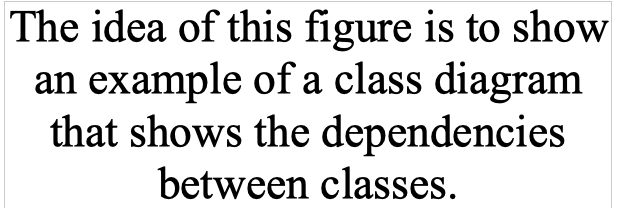
\includegraphics[width=3.4in]{fig/class-diagram-XXX.png}
%	\caption{Class Diagram with Dependencies between JavaScript Classes}
%	\label{fig:class-diagram}
%\end{figure}



\subsection{Considerations}
\label{sec:considerations-vanilla}

In this section we describe some decisions we had to make during the extraction of dependencies from the JavaScript systems presented in Section~\ref{sec:dataset-vanilla}. 
%Basically, we follow the same flowchart presented in Figure~\ref{fig:proposed-approach}. However, during the experiments with systems originally written in JavaScript, instead of transpiled code, we had to deal with different programming styles that required some adaptations, as follows: 

\vspace{2.0 mm}

\noindent \textit{Associations with attributes of type Array.} When we have an attribute of type \textit{Array} whose elements are class instances, this attribute counts as one association only, independently of the number of elements it contains. Listing~\ref{lst_association_array} shows an example in the class \mcode{Graphics}, system {\sc pixi.js}, in which the attribute \mcode{graphicsData} (line 11) is an array that receives instances of \mcode{GraphicsData}. In our analysis, the number of elements in \mcode{graphicsData} do not matter and the attribute counts as one association.

\begin{lstlisting}[caption=Example of association in class \mcode{Graphics} in system {\sc pixi.js}, label=lst_association_array, emph={[2]graphicsData},emphstyle={[2]\ttfamily\bfseries\color{darkgreen}}]
const data = new GraphicsData(
  this.lineWidth,
  this.lineColor,
  this.lineAlpha,
  this.fillColor,
  this.fillAlpha,
  this.filling,
  shape
);
// Adding a class object in an attribute of type Array
this.graphicsData.push(data);

\end{lstlisting} 

\vspace{1.0 mm}

In Section \ref{sec:rq3-recall-results}, Listing~\ref{lst_array_inversifyjs}, we showed an example in which Flow was not able to infer the types of the objects added in the attribute of type array. This is not the case of the code in Listing~\ref{lst_association_array}, in which the class association could be properly identified.

\vspace{2.5 mm}

\noindent \textit{Multiple Types.} Flow is able to infer multiples types for the same property when this property receives different types of objects during execution. For example, in Listing~\ref{lst_association_array}, the parameter \mcode{shape} (line 8) can assume any one of the following types:  \mcode{Circle} $\vert$ \mcode{Ellipse} $\vert$ \mcode{Polygon} $\vert$ \mcode{Rectangle} $\vert$ \mcode{RoundedRectangle}. In our analysis, it means that we have a \aspas{uses} dependency from class \mcode{Graphics} to each one of these possibilities.

%After applying Flow to infer types, we can see in Listing~\ref{lst_association_array} that the parameter \mcode{shape} (line 8) can assume any one of the following types:  \mcode{Circle} $\vert$ \mcode{Ellipse} $\vert$ \mcode{Polygon} $\vert$ \mcode{Rectangle} $\vert$ \mcode{RoundedRectangle}. In our analysis, it means that we have a \aspas{uses} dependency from class \mcode{Graphics} to each one of these possibilities.

\vspace{2.5 mm}

\noindent \textit{Using wildcards to import multiple files at once.} Listing~\ref{lst_import_wildcard} shows an example of an import statement that includes all files inside the indicated folder. In this case, to know which classes from folder \mcode{'../core'} are been used, we perform the following steps:

\vspace{3.5 mm}

\begin{lstlisting}[caption=Example of import statement using wildcard in class \mcode{AccessibilityManager} in system {\sc pixi.js}, label=lst_import_wildcard, emph={[2]graphicsData},emphstyle={[2]\ttfamily\bfseries\color{darkgreen}}]
// Import statement
import * as core from '../core';
...
// Using class 'CanvasRenderer' from package (folder) 'core'
core.CanvasRenderer.registerPlugin('accessibility', AccessibilityManager);

\end{lstlisting} 

%* Inside AccessibilityManager.js, we have an import of multiple files using '*':
% In this case, to know which classes from '../core' are been used, we have to 
\begin{enumerate}
	\item Look for occurences of the prefix \mcode{core} in the source code file, like the one in the beginning of line 5.
	\item Import the related classes, like class \mcode{CanvasRenderer} in line 5.
	\item Eliminate the prefix. After this, the code in line 5 will look like the following:  \mcode{CanvasRenderer.registerPlugin('accessibility'},\\ \mcode{AccessibilityManager);}
\end{enumerate}

\vspace{2.5 mm}

\noindent \textit{Extra features.} We may miss eventual dependencies added by extra features (i.e. features added at runtime) when they are implemented in separated files. For example, class \mcode{DisplayObject}, in system {\sc pixi.js}, is \aspas{extended} in a file called \mcode{cacheAsBitmap.js}, which adds new methods to the class. In our analysis, we investigate the original implementation of the classes, without these extra features, although it would be possible to consider them if necessary. In previous work~\cite{icsr2017}, we have already identified the presence of extra features in system {\sc pixi.js}. 
%Ex: class DisplayObject is "extended" in file cacheAsBitmap.js (CacheData-flow.js).


%*we have some global function, like 'function uploadBaseTextures(prepare, item)' in file CanvasPrepare.js, which are implemented outside the %body of the class only not to be exported to other files, meaning that they work as "private" functions. In this study, we are considering the source could of these functions when looking for dependencies, because they are part of the class implementation.


\begin{comment}

\section {Discussion and Lessons Learned}
\label{sec:discussion}

We started by conducting a study to evaluate the usage of Flow to detect dependencies between classes in legacy JavaScript systems. We could not find any class-to-class dependencies when Flow is used in its default configuration, as in RQ \#1. The reason is that Flow cannot infer types for references across modules. In the analyzed systems, these modules were imported by calling the function \mcode{require}, which is part of \mcode{CommonJS} module specification. In these cases, the imported modules are assigned to variables for further use, as showed when investigating the first research question. As a result, the types of these variables are unknown. To overcome this problem, we decided to replace the variables that make reference to constructor functions implemented in other modules by the names of the respective constructor functions. To achieve this, we expanded the source code imported by the \mcode{require} statements, gathering the classes that depend on each other in the same module (file). This last approach achieved the best results for precision and recall. Finally, we manually analyzed and categorized all false negatives identified in our study, considering RQ \#2. 

It is known that, in both languages, TypeScript and JavaScript, it is possible to implement multiple classes in one file. In theses cases, we understand that the results would be the same for RQ \#1 and RQ \#2. However, in the analyzed systems, we had each class implemented in a different file.

Then, in Section \ref{sec:study-design-vanilla}, we present a study proposed to evaluate the usage of Flow to detect dependencies in vanilla JavaScript systems. The idea is to verify the applicability of using Flow to detect class dependencies in code that is not automatically generated, like in the first study that used TypeScript transpiler to generate JavaScript legacy code. The dataset was composed of systems implemented according to ES6 class syntax to favor the use of name typing to infer types. Basically, we follow the same flowchart presented in Figure~\ref{fig:proposed-approach} to locate dependencies. However, during the experiments with systems originally written in JavaScript, instead of transpiled code, we had to deal with different programming styles that required some adaptations, as described in Section~\ref{sec:considerations-vanilla}. 

Due to the dynamic nature of JavaScript, we hypothesize that it would be necessary to combine static and dynamic analysis to tackle the identified causes of false negatives, improving recall and providing more reliable information. However, it is known that dynamic analysis brings a new set of challenges to software engineers, such as code instrumentation and the need to set up and execute every program under analysis. Therefore, we conclude that the use of Flow to statically infer types and spot class-to-class dependencies in JavaScript legacy code can achieve an accuracy sufficient to support its usage by reverse engineering tools. However, we need to expand the source code in the \mcode{require} statements and to eliminate variable references to classes implemented in other files.

\end{comment}


%:%%%%%%%%%%%%%%%%%%%%%%%%%
\section{Threats to Validity}
\label{sec:threats}

\noindent \textbf{External Validity.} We analyzed seven open-source JavaScript / TypeScript systems in our two studies. For this reason, our results might not represent all possible cases of class dependencies and associations. If other systems are considered, the effect of removing references to classes implemented in other modules can vary. To allow the replication of our study, the oracle along with the detected dependencies for the analyzed systems is available on-line.\footnote{We temporarily omitted this link in accordance with the double-blind submission}
%\footnote{\url{https://github.com/leonardo-silva/JSClassDependencies}} 

Other external validity is related to the fact that we only address module dependencies that comply with \mcode{CommonJS}. We acknowledge that there are different strategies to incorporate modules into JavaScript programs, \emph{e.g.},~ global functions and AMD (Asynchronous Module Definition), which also support modules.

\vspace{1.5 mm}

\noindent \textbf{Internal Validity.} In the first study, we analyze JavaScript legacy code automatically generated by the TypeScript's transpiler. Perhaps the use of a typed language can favor simpler and less dynamic applications. To overcome this threat, we conducted a second study using applications originally implemented in JavaScript. 

\vspace{1.5 mm}

\noindent \textbf{Construct Validity.} We manually inspect the JavaScript /\ TypeScript systems looking for types representing classes. It is possible that we miss dependencies during this inspection. 
%However, the analyzed systems are not large, and, since the types are explicit in the source code, we claim that the oracle contains all class-to-class dependencies.  



%:%%%%%%%%%%%%%%%%%%%%%%%%%
\section{Related Work}
\label{sec:related-work}

In a previous work~\cite{sanerera2017}, we originally introduced the idea of using Flow, a static type-checker for JavaScript, to infer class-to-class associations and dependencies of type \textit{uses} in legacy JavaScript code. They report a preliminary study on two open-source projects whose code is transpiled from TypeScript to JavaScript. They manually annotate import statements with type information in order to infer types for classes. Their results show that precision reaches 100\% in the two evaluated systems. However, recall is lower, ranging from 37\% to 51\% for all dependencies, which is probably not sufficient to provide reliable reverse engineering tools to JavaScript developers. In this paper, we also use Flow to infer types that correspond to class references, but with a different strategy. We expand the source code in the \mcode{require} statements to eliminate variable references to class constructor functions implemented in other modules. In a first study, we analyzed the same TypeScript systems they used in their study, {\sc inversifyjs} and {\sc satellizer}, plus another system called {\sc xstream}. Our results show that precision continues in 100\% in the three evaluated systems. Flow's recall increases, 80\% - 98\% for all dependencies, including associations and dependencies of type \aspas{uses}.

Gao et al.~\cite{Gao2017} investigate the benefits of using static type systems, notably Facebook's Flow and Microsoft's TypeScript, to detect public bugs. For the analyzed systems, they select a fixed bug and check out the code just prior to the fix. They manually add type annotations to the buggy code and test whether Flow and TypeScript report an error. They then report the proportion of bugs on which these type systems reported an error. The conclusion is that both static type systems find an important percentage of public bugs: 15\% each. Moreover, they state that the use of such type systems can bring other benefits, such as facilitating code search/completion and serving as documentation.

Rostami et al.~\cite{rostami2016} propose an alternative tool, called JSDeodorant, to detect constructor functions in legacy JavaScript systems. They first identify all object instantiations, even when there is no explicit object instantiation statement (\emph{e.g.,} the keyword \mcode{new}), and then link each instance to its constructor function. Finally, the identified constructors represent the emulated classes and the functions that belong to these constructors (inner functions) represent the methods.

Cloutier et al.~\cite{wavi2016} present a reverse engineering tool, called WAVI, that uses static analysis and a filter-based mechanism to retrieve and document the structure of a Web
application. WAVI provides customized class diagrams for JavaScript, as proposed by web application extensions (WAE)~\cite{wae-conallen-2002}. However, the tool is not able to identify class constructors nor their dependencies in legacy JavaScript code. 

Jensen et al.~\cite{tajs2009,lazypropagation2010} introduce TAJS, which is a dataflow analyzer for JavaScript that relies on allocation site abstraction for objects and constant propagation for primitive values. The authors also provide an Eclipse plug-in that can be used to catch type-related errors. Therefore, future work can extend our study using TAJS as type inferencer.

There are also tools and techniques that rely on execution traces to understand event-based interactions in JavaScript. Alimadadi et al.~\cite{clematis2014} presented a tool, called Clematis, for supporting comprehension of web applications. The tool captures a detailed trace of a web application's behaviour during a particular user session and creates a behavioural model through a combination of automated JavaScript code instrumentation and transformation. This model is then presented to the developers as an interactive visualization that depicts the creation and flow of triggered events. Zaidman et al.~\cite{zaidman-2013} presented a tool, called FireDetective, to record execution traces of the JavaScript code that is executed in the browser (client) and also in the server. The level of detail used is the call level: the tool records the names of all functions and methods that were called, and in what order they were called, allowing the reconstruction of a call tree representation of each trace. Although event-based interactions do not involve class relations directly, future work can use similar techniques to extend our approach by looking for dependencies in execution traces. 


%:%%%%%%%%%%%%%%%%%%%%%%%%%
\section{Conclusion and Future Work}
\label{sec:conclusion}

In this paper, we evaluate the usage of Flow, a static type-checker for JavaScript, to infer class-to-class associations and dependencies of type \aspas{uses} in legacy JavaScript code. We report a study on three open-source projects whose code is transpiled from TypeScript to JavaScript. We could not find any class-to-class dependencies when Flow is used in its default configuration, as in the first research question. After expanding the source code in the \mcode{require} statements to eliminate variable references to class constructor functions implemented in other modules, our results show that precision reaches 100\% in the evaluated systems. Flow's recall ranges from 85\% to 96\% for associations, 64\% to 99\% for \aspas{uses} dependencies, and, if we consider both, from 80\% to 98\%. We manually analyzed and categorized all false negatives identified in our study. These false negatives are due to: (i) use of dependency injection (8 instances); (ii) absence of method invocation (8 instances); (iii) use of the object \mcode{arguments} (10 instances); and (iv) use of attributes of type \mcode{Array} (7 instances). The overall results suggest that this approach can be used to support the implementation of reverse engineering tools for JavaScript. Finally, in a second study, we successfully identify class-to-class dependencies and associations on vanilla JavaScript projects by applying our approach. Although it is not mandatory, the migration of legacy JavaScript code to the ES6 class syntax allows the use of name typing instead of structural typing, simplifying the type inference and, by consequence, the identification of class-to-class dependencies. 

As future work, we plan to extend our study by analyzing a larger set of JavaScript systems. We also intent to investigate the use of our approach to assist developers that intent to migrate their JavaScript systems to a typed version, \emph{e.g.,} TypeScript. Recent reports show that this kind of migration can be a hard and time consuming task~\footnote{\url{https://davidgom.es/porting-30k-lines-of-code-from-flow-to-typescript/}}. Moreover, we may improve recall by combining Flow (or other static analysis tool) with dynamic analysis. We can instrument JavaScript code to record execution traces using, for example, tools like Aran~\cite{aran-2015} or Jalangi~\cite{jalangi2013}. Finally, the class-to-class dependencies can also be used to compute software quality metrics for JavaScript, such as \textit{fanin}, \textit{fanout}, and other source code metrics~\cite{CK_metrics}.

% , including the investigation of systems whose native language is JavaScript

\section*{References}

\bibliography{thesisbib_ist2018}

\end{document}